\section*{Data Sources \& Modeling choices}

The inputs we use to generate our measure of state preference through this tensor regression framework are a score of two countries' UN voting similarity index in year $t$ \citep{voeten:2013}\footnote{Specifically, the ``agree3un'' variable.}, and a count of the number of alliance commitments made by one state to another by time $t$ \citep{gibler:sarkees:2004}. However, to facilitate comparison between the metrics, we first standardize these two measures. This gives us an $n \times n \times 2 \times T$ array, where the first two dimensions represent countries, the third is the particular measure of similarity, and the fourth dimension is the year. The item at index (1,2,1,1) would be the transformed value of the UN similarity index for countries $i$ and $j$ at the first year of our data, similarly (1,2,2,1) would be the number of alliance relationships.

To generate a time series of measurements of $\bl A$ and $\bl B$ we run separate tensor regression models for every year and in each only include the last three years of dyadic observations.\footnote{As a robustness check, we also ran models in which we include the last five years of observations, however, the state preference measurements generated through this choice had worse out-of-sample in terms of predicting conflict.} Thus our measurement of state preference at $t=4$ includes observations from $t=1-3$, $t=5$ would include observations from $t=2-4$, and so on. The risk if we increase the size of the rolling temporal window is that we would be including data that is no longer relevant to a country's relative preferences. For instance, Turkey and Russia's relationship looks a lot more positive when we look at 2013 and 2014 than 2015 following the downing of a Russian warplane by Turkish F-16s in the Turkey-Syria border \citep{bbc:2015}.\footnote{A limitation of the approach that we are using here is that generating a time series of measurements of $\bl A$ and $\bl B$ requires running separate models. There are alternative frameworks that have been developed to allow for time varying dependence parameters. For example, \citet{minhas:etal:2017:arxiv} extend the MLTR framework by allowing it to have time-varying dependence parameters and also model $\bl A$ and $\bl B$ be a function of exogenous covariates. However, for this approach, one must specify a set of exogenous covariates that they think can explain dependencies in relations between dyads. Additionally, some of the other variants that exist in the literature that would allow for the estimation of a time varying set of dependence parameters have so far only been developed for binary networks (e.g., \citealp{durante:etal:2017,park:sohn:2017}).}

Additionally, though we obtain estimates of both $\bl A$ and $\bl B$, we only use estimates of $\bl A$ in generating our measure of state preference. The dyad specific regression coefficients in $\bl A$ capture how similar two countries are in terms of actions that they initiate, whereas $\bl B$ provides us a measurement of how similar countries are in terms of who they receive actions from. Though the latter is of substantive interest, we leave further analysis of it to future research. Measurement of how similar two countries are in terms of the actions that they initiate provides us with a closer measurement of how the foreign policy preferences of two states are aligned as it will be based on the actions that they choose, rather than actions taken by third parties. For convenience in the rest of the paper, we term to the estimates of state preference that we retrieve from $\bl A$ as ``tensor dependence''.

\subsection*{Face Plausibility}

An important question for these different measures of preferences, are whether they give results that ``make sense''. In particular, we would hope that the measure both provides plausible levels to relationships -- sorting states into friends and foes effectively -- and that when these measures change, they do so in ways that correspond to changes in the world. One of our principle critiques of both alliance portfolio S-scores and UN voting based ideal points is that they describe certain important relationships in a way that some may find implausible. Using our measure we return to the example of relationships in East Asia in 2012. We find that our tensor dependence measure, depicted in figure \ref{korea:withus}, corresponds much better to conventional understanding of the relations between these states.

\begin{figure}[ht]
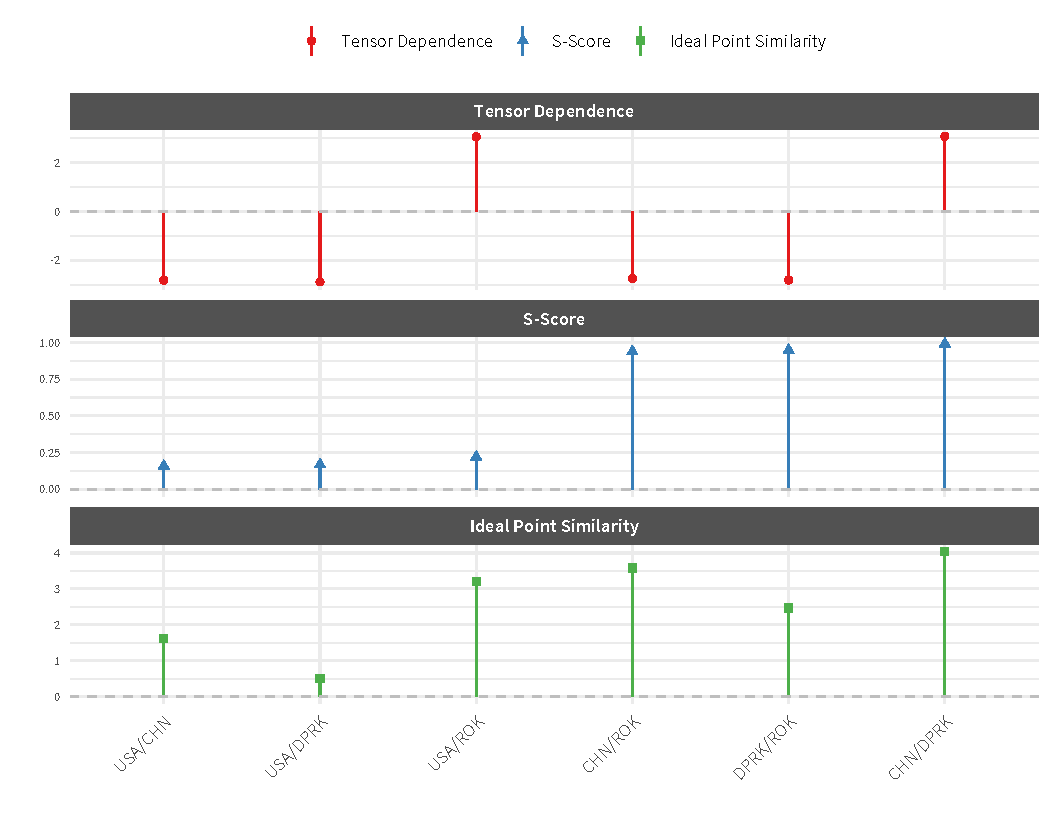
\includegraphics[width=1\textwidth]{idPtScoreLatAngleViz}
\caption{Visualization of tensor dependence, S-score, and ideal point similarity relationships between China (CHN), North Korea (DPRK), South Korea (ROK), and the United States (USA) in 2012. Within each panel a higher score denotes that the countries have a more positive relationship.}
\label{korea:withus}
\end{figure}

To generalize this test of face plausibility, we present all three measures' accounts of six dyadic relationships over time. In each of the plots, we have standardized each of the measures and higher scores denotes that countries have a more positive relationship. We first look at three close relationships where we would expect to see similar preferences. Figure \ref{friendly:dyads} depicts the relationships between France and Germany, the US and Israel, and North Korea and China. In all three cases our tensor dependence measure consistently places each of these relationships on the positive end of the spectrum. S-Scores correctly classify Franco-German and Sino-North Korean friendship, while the US/Israel relationship is characterized as actually quite poor. The ideal points similarity measure largely matches what we find with tensor dependence but shows notably more variation in the quality of these relationships over time.

\begin{figure}
	\centering
	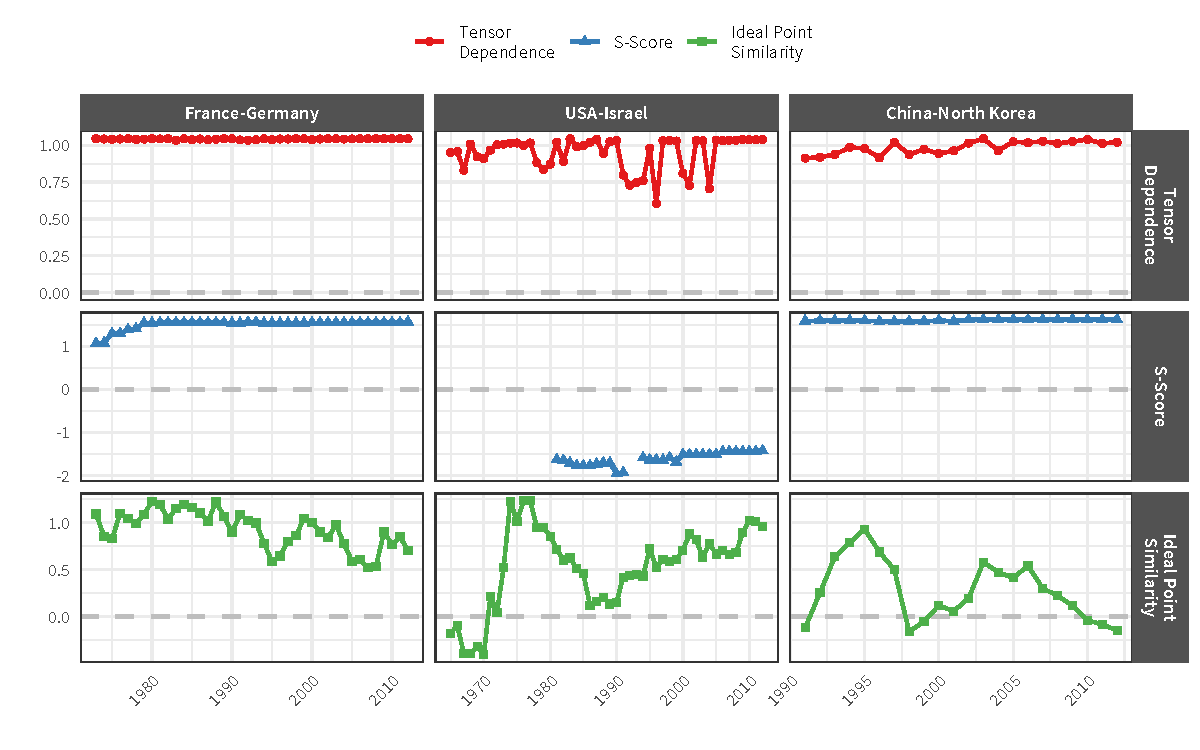
\includegraphics[width=1\textwidth]{plausPlot_1_border}
	\caption{Dyadic relationships between France-Germany, United States-Israel, and China-North Korea according to the different preference measures. Yearly tensor dependence scores between dyads are denoted by red circles, ideal point similarity based on UN voting in blue triangles, and S-scores by green squares. Each of the measures is standardized and within each panel a higher score denotes that the countries have a more positive relationship. The grey dashed line in each of the panels designates a neutral relationship.}
	\label{friendly:dyads}
\end{figure}

In Figure \ref{unfriendly:dyads} we look at the United States' relationship with three countries that are characterized by change and major events. S-scores are the only measure that do not detect a marked improvement in the US/Russian relationship at the end of the Cold War. Both the UN ideal points and tensor dependence measures find significant improvements followed by a drift toward enmity, whereas S-scores have a constant (though slightly improving) neutral relationship. The tensor dependence measure also shows that the US-Russia relationship in the years immediately after the Cold War was actually quite positive. Additionally, the tensor dependence measure for US and Russia does spike in 2010 likely because of Russia joining the US and its allies in placing tighter sanctions on Iran. For the US and Iraq no measure depicts more similar preferences following the US occupation, though only our tensor dependence measure finds a substantial increase in enmity in the run-up to the United States' 2003 invasion. Finally, each of the measures do find that the US relationship with China is quite weak.

\begin{figure}
	\centering
	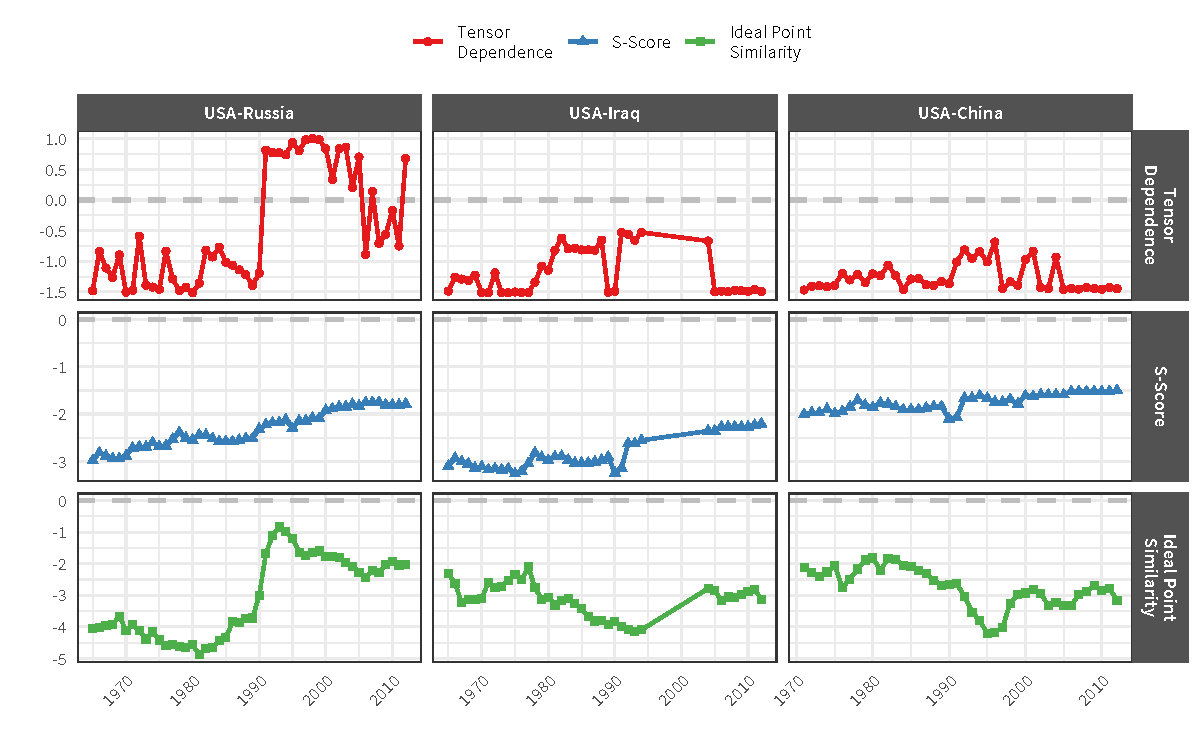
\includegraphics[width=1\textwidth]{plausPlot_2_border}
	\caption{Dyadic relationships between France-Germany, United States-Israel, and China-North Korea according to the different preference measures. Yearly tensor dependence scores between dyads are denoted by red circles, ideal point similarity based on UN voting in blue triangles, and S-scores by green squares. Each of the measures is standardized and within each panel a higher score denotes that the countries have a more positive relationship. The grey dashed line in each of the panels designates a neutral relationship.}
	\label{unfriendly:dyads}
\end{figure}

As can be seen from these relationships, the measure of preferences based on tensor dependence distance is in many cases as plausible or more than incumbent measures of preferences. While the measure has more temporal instability than S-scores or UN ideal points, in these six cases it often does better, and rarely worse at conforming to our expectations of the relationships. Of course, this could just be a case of us picking particularly propitious cases.

\subsection*{Relationship between Tensor Dependence and Components}

We also examine how our tensor dependence measure is affected by changes in alliance relations or UN voting similarity by considering the relationship between the United States and Israel in 1981. With the signing of the ``Joint Memorandum of Understanding," the two states went from having no alliance relationship to having one, the states were voting together at the UN 80\% of the time (up 3\% from 1980, below the median yearly change for this dyad). These factors, coupled with changes in the third order effects for the dyad, led the tensor dependence to increase from about 2.72 to about 3.08.

Of course, another pair of countries might sign an alliance (or withdraw from an alliance) and have a markedly different effect on this measure of tensor dependency. For example, in 1977, the United Kingdom and the United States went from being in 5 alliances together to being in 4, and this led to a drop in their tensor dependence from 3.13 to 2.28, despite a decrease in their UN voting similarity of less than 1\%. This is because the alliance that ended in 1977 was the Southeast Asian Treaty Organization, which had 4 other members, and so the third order effects were concomittantly more severe. To capture the aggregate effects of dyadic variables on our measure of tensor dependence, we estimate a simple AR(1) model, depicted in Table~\ref{tensor:ols}, and these dyadic factors account for about 78\% of the variance, with the rest coming from third order factors. Next, we conduct a the large-N analysis of conflict and compare the added utility of these various measures of state preferences.

\begin{table}[ht]
	\centering
	\begin{tabular}{lcccc}
		\hline
		& Estimate & Std. Error & t value & Pr($>|t|$) \\
		\hline
		(Intercept) & 0.0773 & 0.001 & 74.26 & 0.000 \\
		Tensor Dependence$_{t-1}$ & 0.888 & 0.0004 & 2094.81 & 0.000 \\
		Change in Alliance Relationship & 0.131 & 0.009 & 15.30 & 0.000 \\
		Change in UN Voting Similarity & 4.401 & 0.014 & 313.14 & 0.000 \\
		\hline
	\end{tabular}
	\caption{Regression of tensor dependence on dyadic components.}
	\label{tensor:ols}
\end{table}

\subsection*{Model Competition}

To evaluate the different measures of state preferences, we assess their utility in predicting the occurrence of interstate disputes. Here we look at four non-nested models: a model using no measures of state preferences, one using an S-Score based on similarity in alliance portfolio \citep{signorino:ritter:1999}, one using the ideal points determined by UN voting \citep{bailey:etal:2015}, a model using both UN ideal points and alliance S-scores, and finally, a model using our tensor dependence approach that combines the raw data from UN voting and alliances. We evaluate the models on two criteria: whether state preferences have a consistent effect in the predicted direction, and how well each model does at predicting disputes in an out-of-sample context.

In each of these models, we utilize a logistic regression of Militarized Interstate Dispute (MID) participation on measures of state preferences and a vector of control variables. These control variables overlap with the standard framework used in O'Neal and Russett's canonical work on the democratic peace \citep{oneal:russett:1997}.\footnote{The exception is that our models ignore trade interdependency, as including that data drastically decreases the number of observations.} In particular, we include a binary measure of joint democracy (whether both states have Polity IV scores $\geq 7$), whether the states are contiguous, and the ratio of state capabilities as measured by the Correlates of War Project's Composite Index of National Capabilities (CINC). We also account for temporal interdependence using a peace year spline \citep{carter:signorino:2010}.

\subsection*{In-sample explanation}

As detailed in figure \ref{fig:coefP}, two of the measures of state preferences perform as we would expect.\footnote{Given that our estimate of $\bl A$ comes with uncertainty, we also ran our analysis using several different draws from the distribution for $\bl A$, when combining these estimates via \citet{rubin:1976}'s rules, we found results similar to what is shown below.}  Our measure of state preference using tensor dependence difference is significant and negative: states that are more similar to one another based on our measure are less likely to engage in conflict. Similarly, UN ideal point similarity passes this test. The measure using UN voting ideal points is negative and clearly distinct from $0$, indicating that states with higher levels of similarity in terms of UN voting are less likely to find themselves in conflict. On the other hand, higher alliance S-scores are consistently associated with higher probabilities of conflict -- so states with more similar preferences as measured using alliance portfolios are more likely to quarrel. This is, to say the least, surprising. These results hold when those measures of preference are used in isolation, or in tandem. The effects of the control variables are consistent when using differing versions of state preference and also generally align with the extant literature.

% The models have one major difference in terms of the controls: in the model using tensor dependence distance, joint democracy is indistinguishable from $0$. This is particularly interesting as one of the major criticisms of democratic peace theory is that democracies have similar preferences. Some argue that it is similarity in preferences that leads to peace among democracies.  Despite this dispute, most attempts to include preferences in the standard democratic peace regressions still find a consistent pacifying effect of democracy. (as do those models with UN voting and S-scores presented here). %With our measure of preferences, however, democracy's effect is negligible. More research is necessary to disentangle whether the criticism is now credible, but work such as this provides a template for us to parse out the effect of democracy versus preferences on conflict.


\begin{figure}[ht]
	\centering
	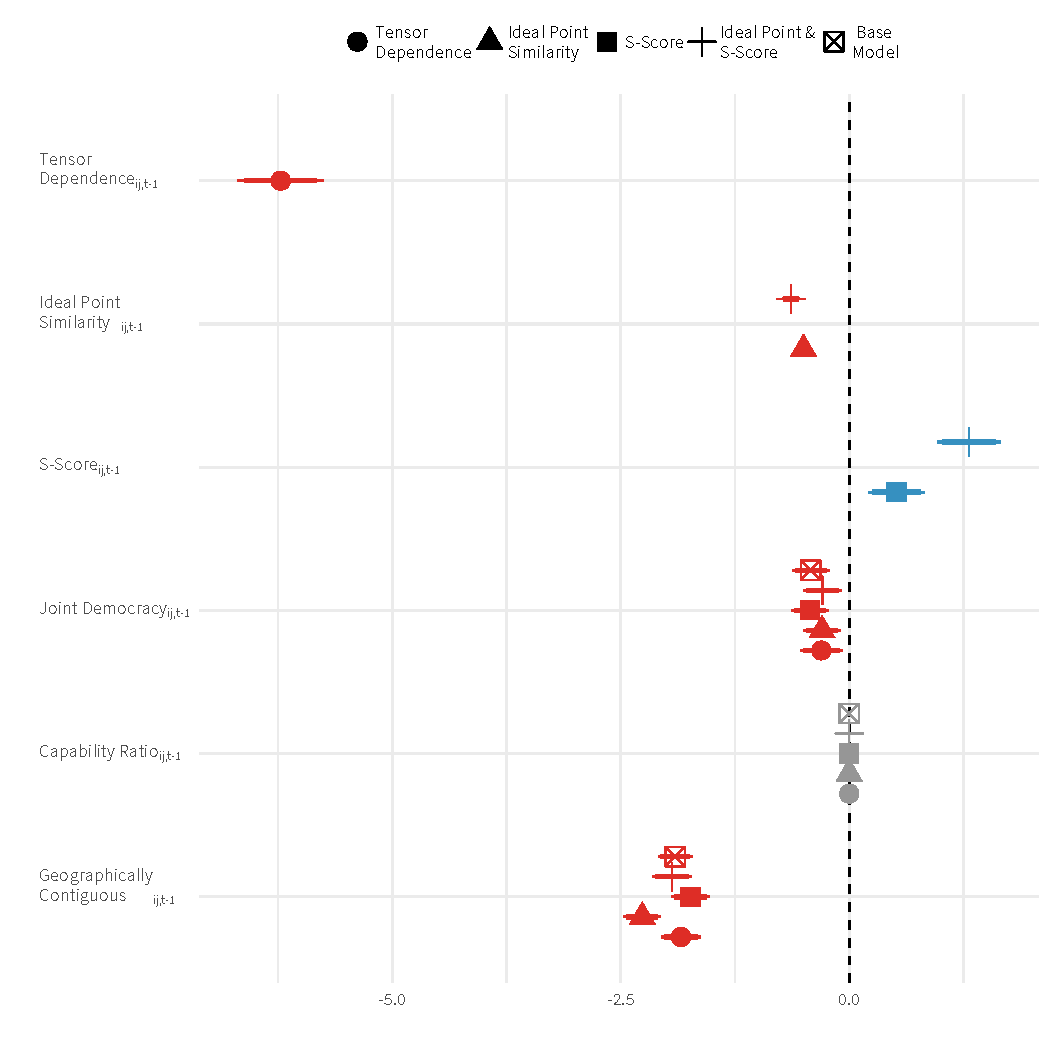
\includegraphics[width=.7\textwidth]{betaEst}
	\caption{Parameter estimates from models with different measures of state preference. Point represents average estimate, line through the point represents the 95\% confidence interval.}
	\label{fig:coefP}
\end{figure}
\FloatBarrier

\subsection*{Out-of-sample prediction}

Given these results, we can say that two of the measures of preferences behave as we would expect, while S-scores do not. To adjudicate between the two measures of preference similarity that pass this test, and help determine what we should make of the differing effect of democracy, we turn to out-of-sample prediction. We undertake a cross-validation procedure in which we partition our data into 30 different folds. This process works by taking each fold, $k$, and running a logistic model excluding data from that fold. Once we have parameter estimates from a model that excluded fold $k$, we predict the probability of a MID in fold $k$ using only the parameter estimates and the covariates from fold $k$.

We then compare the performance of these models using two metrics: area under the Receiver Operator Characteristic Curve (AUC-ROC) and the Precision Recall Curve (AUC-PR). The ROC curve examines the tradeoff between true positives and false positives, and the PR examines the tradeoff between making only correct predictions and predicting all the disputes that occurred. In general, the ROC will disproportionately reward those models that predict $0$ well -- and we can interpret the ROC as the likelihood a prediction is correct. The numeric value for the PR has less of a clear interpretation, but models with a higher PR do a better job of predicting when events actually occur.

As shown in figure \ref{fig:roc}, the model using tensor dependence distance decisively outperforms the other models. While the AUC-ROC is somewhat higher with the tensor dependence model, the real difference between the measures shines through in the AUC-PR, where the model using this measure performs almost twice as well as the base model. In contrast, models using other measures of state preferences yield only minimal improvements in prediction over the base model. This is especially relevant because AUC-PR specifically focuses on the difficult task of predicting conflict, compared to the relatively easier task of predicting non-conflict that is rewarded by the AUC-ROC measure. Thus we have reason for confidence in both the usefulness of this measure of state preferences.

\begin{figure}[ht]
	\centering
	\begin{tabular}{cc}
	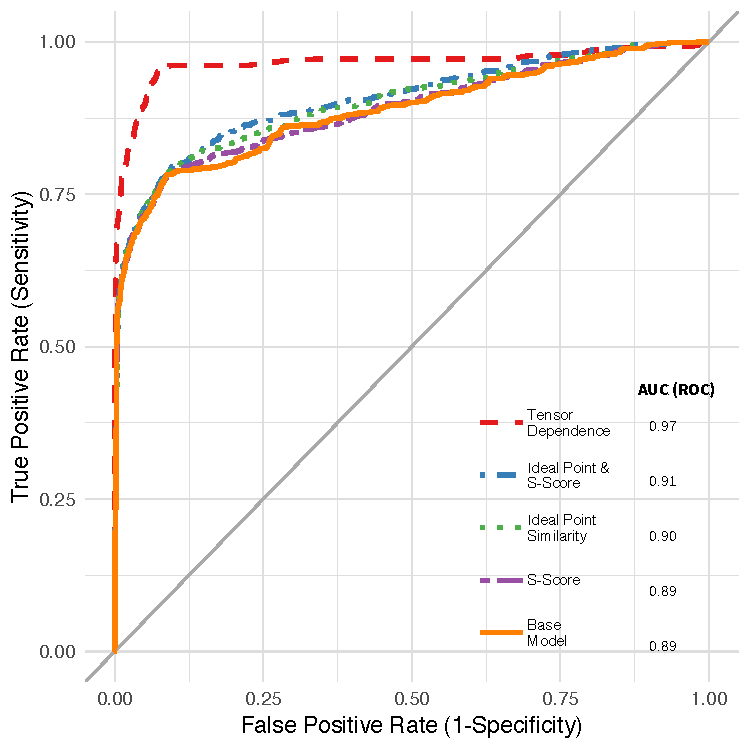
\includegraphics[width=.4\textwidth]{roc_outSample} &
	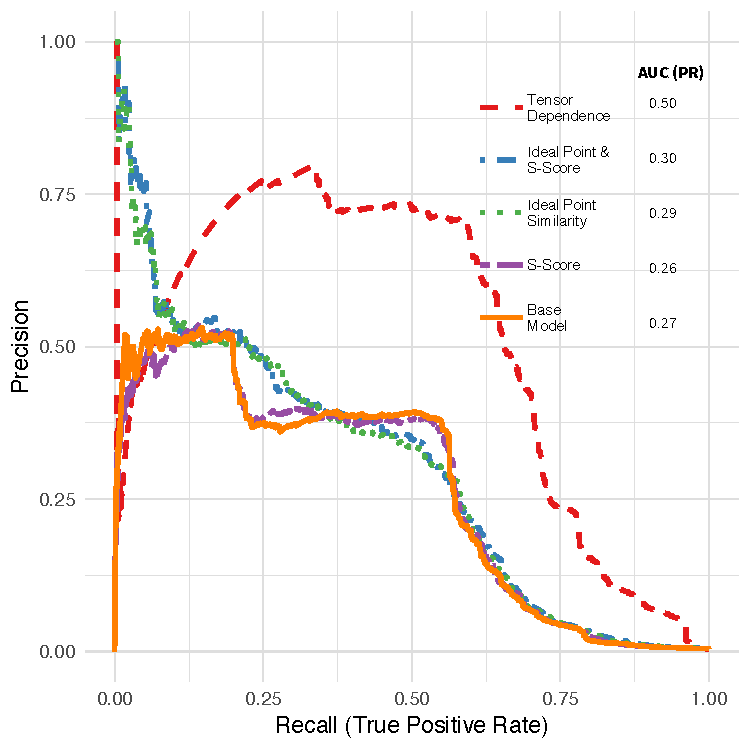
\includegraphics[width=.4\textwidth]{rocPr_outSample}
	\end{tabular}
	\caption{Assessments of out-of-sample predictive performance using ROC curves and PR curves. AUC statistics are provided as well for both curves.}
	\label{fig:roc}
\end{figure}
\FloatBarrier
